Form�let med fors�get er, at finde en musesensor der vil kunne opfange bilens hastighed. For at finde ud af om musesensoren kan opfange bilens hastighed, m� nogle fors�g foretages. Hvis bilens maxhastighed er 6m/s, og den musesensor, der er tilt�nkt projektet, kun kan opfange 5m/s, m� en ny musesensor findes. For netop at finde den rigtige musesensor, m� disse fors�g derfor foretages.
\subsubsection*{Fors�gsopstilling}
\begin{figure}[htb]
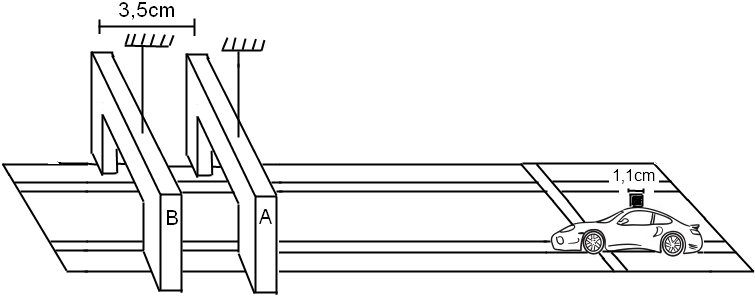
\includegraphics[scale=0.5]{hastighed3.png}
\caption{Hastighedsopstilling}
\label{hastighed}
\end{figure}
Bilen startes ved den hvide streg og f�r givet max hastighed. N�r bilen er i max hastighed, er en fotocelle opstillet, til at m�le dens hastighed. P� bilens tag er monteret en sort boks (som ses p� figur \ref{hastighed}). Fotocellen m�ler tiden det tager den sorte boks at pasere A, B og fra A til B (Kaldet AB). M�den hastigheden beregnes p�, er ved simpel matematisk udregning. Ved at tage et par fors�g og med tro p� at fotocellen fungere, kan dette fors�g siges at v�re fejlfrit. \\
F�lgende tabel er de seks fors�g, der er blevet udf�rt. 
\begin{table}[htb]
\begin{center}
	\begin{tabular}{| l | l | l | l|}
			\backslashbox{Fors�g}{Placering} & A (ms) & B (ms) & AB (ms)\\
			\hline
			1 & 2.68 & 2.60 & 85.91\\
			2 & 2.69 & 2.70 & 86.42\\
			3 & 2.55 & 2.58 & 82.27\\
			4 & 2.57 & 2.57 & 82.25\\
			5 & 2.53 & 2.50 & 80.83\\
			6 & 2.55 & 2.55 & 81.93\\
		\end{tabular}
\end{center}
	\caption{Hastighedsm�leresultater}
	\label{tab:hastighed} %%ref
\end{table} \\
Som tidligere n�vnt, kan hastigheden findes ved hj�lp af simple matematiske beregninger. Der er udvalgt tilf�ldigt i fors�gene og afstanden er delt med tiden. Det kan virke overfl�digt at tage seks udregninger med, men for at vise fors�gene n�sten er identiske, er dette alligevel valgt. 
\begin{align*}
Hastighed&=\frac{Afstand}{Tid} = \frac{1.1\cdot 10^{-2}m}{2.53 \cdot 10^{-3}s} = 4.35 \frac{m}{s}\\
Hastighed&=\frac{Afstand}{Tid} = \frac{1.1\cdot 10^{-2}m}{2.50 \cdot 10^{-3}s} = 4.40 \frac{m}{s}\\
Hastighed&=\frac{Afstand}{Tid} = \frac{1.1\cdot 10^{-2}m}{2.55 \cdot 10^{-3}s} = 4.31 \frac{m}{s}\\
Hastighed&=\frac{Afstand}{Tid} = \frac{350\cdot 10^{-3}m}{80.83 \cdot 10^{-3}s} = 4.33 \frac{m}{s}\\
Hastighed&=\frac{Afstand}{Tid} = \frac{350\cdot 10^{-3}m}{81.93 \cdot 10^{-3}s} = 4.27 \frac{m}{s}
\end{align*}
Fors�get er udf�rt uden top-karosset monteret p� bilen og bilen vil derfor aldrig kunne opn� denne max hastighed - da v�gten er betydelig mindre. Konklusionen p� dette fors�g er, at hvis musesensoren kan opfange mere end 4.40m/s, er det mere end rigeligt.